\documentclass[12pt,a4paper]{article}
\usepackage[utf8]{inputenc}
\usepackage[T1]{fontenc}
\usepackage[brazil]{babel}
\usepackage[a4paper,margin=2.5cm]{geometry}
\usepackage{graphicx}
\usepackage{booktabs}
\usepackage{amsmath}
\usepackage{float}
\usepackage[round,authoryear]{natbib}
\usepackage[hidelinks]{hyperref}
\graphicspath{{../outputs/figures/}}
\setlength{\parskip}{0.4em}
\renewcommand{\arraystretch}{1.15}

\title{\textbf{Exposição das gestoras a ações:\\ generalização para todas as ações} \\[0.4em]
\large Documento complementar ao TCC, com extensão exploratória de de-duplicação fundo-sobre-fundo}
\author{João Paulo Zangrandi \\ \small Orientador: Prof.\ Maurício Ferraresi Junior --- FGV EESP}
\date{\today}

\begin{document}

\begin{titlepage}
\centering
\vspace*{1.5cm}
{\scshape\large Fundação Getulio Vargas --- EESP\par}
\vspace{2.5cm}
{\huge\bfseries Exposição das gestoras a ações\par}
\vspace{0.6cm}
{\Large Generalização do piloto ITUB4 para \textbf{todas as ações} (2016--2021) e extensão exploratória com CDA\par}
\vspace{3cm}
{\Large João Paulo Zangrandi\par}
\vspace{0.4cm}
{\large Orientador: Prof.\ Maurício Ferraresi Junior\par}
\vfill
{\large São Paulo --- \today\par}
\end{titlepage}

\section*{Resumo}
\addcontentsline{toc}{section}{Resumo}
Este documento complementa o TCC (que validou o método com ITUB4) \textbf{generalizando a análise para todas
as ações} detidas pelos fundos da amostra (2016--2021). Reaplicamos o mesmo \emph{pipeline} central ---
exposição em valor (R\$/US\$), definição net, grupos econômicos consolidados, FICs mantidos --- a
\textbf{836 ações}, produzindo um painel gestora $\times$ mês $\times$ ticker com 381.512 observações. O
resultado central do painel é a \textbf{concentração} da demanda institucional: as ações detidas por
\textbf{todas} as 42 gestoras são as \emph{blue chips} do índice (VALE3, PETR4, ITUB4, BBDC4\ldots), o que
conecta diretamente com a fragilidade de preços de \citet{greenwoodthesmar2011}. Como extensão
\textbf{exploratória}, usamos a CDA Bloco~2 para medir dupla contagem interna entre fundos da mesma gestora:
a exposição total em ações cai de R\$\,14,3 tri (bruta) para R\$\,8,9 tri (de-duplicada), uma duplicação
interna de \textbf{37,4\%}. Esse resultado é informativo, mas deve ser mantido como complementar até o uso da
CDA ser validado no desenho do TCC.

\noindent\textbf{Palavras-chave:} exposição de gestoras; concentração de propriedade; demand-based asset
pricing; fundo-sobre-fundo; CDA.

\newpage
\tableofcontents
\newpage

\section{Introdução}\label{sec:intro}
O TCC validou, com \textbf{ITUB4}, um método para medir a exposição das gestoras a ações (ver documento
principal). Este complemento responde à pergunta natural: \emph{o que se observa quando estendemos para
todas as ações?} A pergunta principal é a concentração da demanda institucional por ação. A de-duplicação
fundo-sobre-fundo é analisada em separado como extensão exploratória com CDA, não como premissa do painel
central.

A motivação teórica é a mesma --- \emph{demand-based asset pricing} \citep{koijenyogo2019,gabaixkoijen2021} e
fragilidade de preços por propriedade comum \citep{greenwoodthesmar2011}. Medir, para todas as ações, quanto
da exposição agregada é ``inflada'' por participações sobre participações é um passo direto para discutir
risco sistêmico.

\section{Dados e método (resumo)}\label{sec:metodo}
Reutilizamos integralmente o \emph{pipeline} central do TCC (base CONS para \emph{holdings}; base SH para
gestora e PL), descrito no documento principal. A CDA Bloco~2 entra somente na extensão de de-duplicação. As
mudanças principais:
\begin{itemize}
\item \textbf{Todos os tickers}, não só ITUB4: o ticker é extraído do fim do \texttt{Nome\_Ativo}
(regex \texttt{[A-Z]\{4\}[0-9]\{1,2\}\$}), e a variante (direta/cedida/obrigações) é classificada por
palavra-chave --- exatamente como no piloto, agora para todas as linhas.
\item \textbf{De-duplicação exploratória} generalizada. Para a exposição \emph{total} em ações, seja $E_i$ a
exposição consolidada do fundo $i$ (soma de todas as ações, net). Removendo a sobreposição interna (mesma gestora),
\[ \text{dedup}_g = \sum_{i\in g} E_i - \!\!\sum_{A\to B\;\text{em }g}\!\! \phi_{A\to B}\,E_B,
   \qquad \phi_{A\to B} = \frac{v_{A\to B}}{PL_B}, \]
e o mesmo, por ação, trocando $E$ por $L^{(ticker)}$.
\end{itemize}

\section{Resultados}\label{sec:result}

\paragraph{Cobertura.} Das linhas da CONS (todas ``Ações''), \textbf{99\%} têm um ticker reconhecível (o
restante são ações de companhia fechada, sem código de negociação). Ao todo, \textbf{836 tickers} distintos;
o painel gestora $\times$ mês $\times$ ticker tem \textbf{381.512} observações (42 grupos, 72 meses).

\paragraph{Extensão CDA: duplicação interna ($\approx 37\%$).} A Tabela~\ref{tab:dedup_g} mostra a exposição
\emph{total} em ações por gestora, bruta vs de-duplicada, na extensão com CDA. No agregado, a exposição cai de
R\$\,14,3 tri para R\$\,8,9 tri --- \textbf{37,4\% de dupla contagem interna}, quase idêntico ao valor do
ITUB4 (37,6\%). O fenômeno se repete \textbf{ação a ação} (Tabela~\ref{tab:dedup_t} e
Figura~\ref{fig:dedupstock}): quase todas as \emph{blue chips} ficam entre 30\% e 42\%. A leitura correta é
condicional: se a CDA for aceita como extensão metodológica, ITUB4 não era especial na duplicação interna.

\begin{table}[H]\centering
\caption{Exposição TOTAL em ações por gestora: bruta vs de-duplicada (média mensal, R\$ bilhões).}
\label{tab:dedup_g}
\small
\begin{tabular}{lrrr}
\toprule
\textbf{Gestora} & \textbf{Bruta (R\$ bi)} & \textbf{De-dup (R\$ bi)} & \textbf{Dupla cont.} \\
\midrule
Itaú                   & 43,8 & 24,9 & 41,4\% \\
Bradesco               & 14,2 & 10,0 & 30,3\% \\
BB                     & 12,7 &  8,5 & 31,0\% \\
Atmos Capital          & 10,0 &  5,1 & 48,6\% \\
BTG Pactual            &  9,9 &  7,3 & 35,0\% \\
Truxt Investimentos    &  9,9 &  4,5 & 52,4\% \\
Safra                  &  8,7 &  5,2 & 37,9\% \\
Caixa                  &  6,3 &  5,9 &  4,2\% \\
\midrule
\textbf{Agregado}      & \textbf{37,4\% de dupla contagem} & & \\
\bottomrule
\end{tabular}
\end{table}

\begin{table}[H]\centering
\caption{Dupla contagem interna por ação (maiores exposições). Bruto $=$ soma 2016--2021.}
\label{tab:dedup_t}
\small
\begin{tabular}{lrr|lrr}
\toprule
\textbf{Ação} & \textbf{Bruto (R\$ bi)} & \textbf{Dupla c.} & \textbf{Ação} & \textbf{Bruto (R\$ bi)} & \textbf{Dupla c.} \\
\midrule
VALE3 & 758 & 37,1\% & ITSA4  & 290 & 33,9\% \\
PETR4 & 657 & 36,6\% & BPAC11 & 237 & 41,8\% \\
ITUB4 & 497 & 37,6\% & SUZB3  & 222 & 36,6\% \\
BBDC4 & 448 & 37,0\% & PETR3  & 179 & 38,5\% \\
EQTL3 & 431 & 36,7\% & ABEV3  & 159 & 40,7\% \\
BBAS3 & 348 & 30,0\% & JBSS3  & 144 & 41,5\% \\
RENT3 & 329 & 41,1\% & GGBR4  & 136 & 41,6\% \\
LREN3 & 325 & 39,9\% & RADL3  & 100 & 40,9\% \\
\bottomrule
\end{tabular}
\end{table}

\begin{figure}[H]\centering
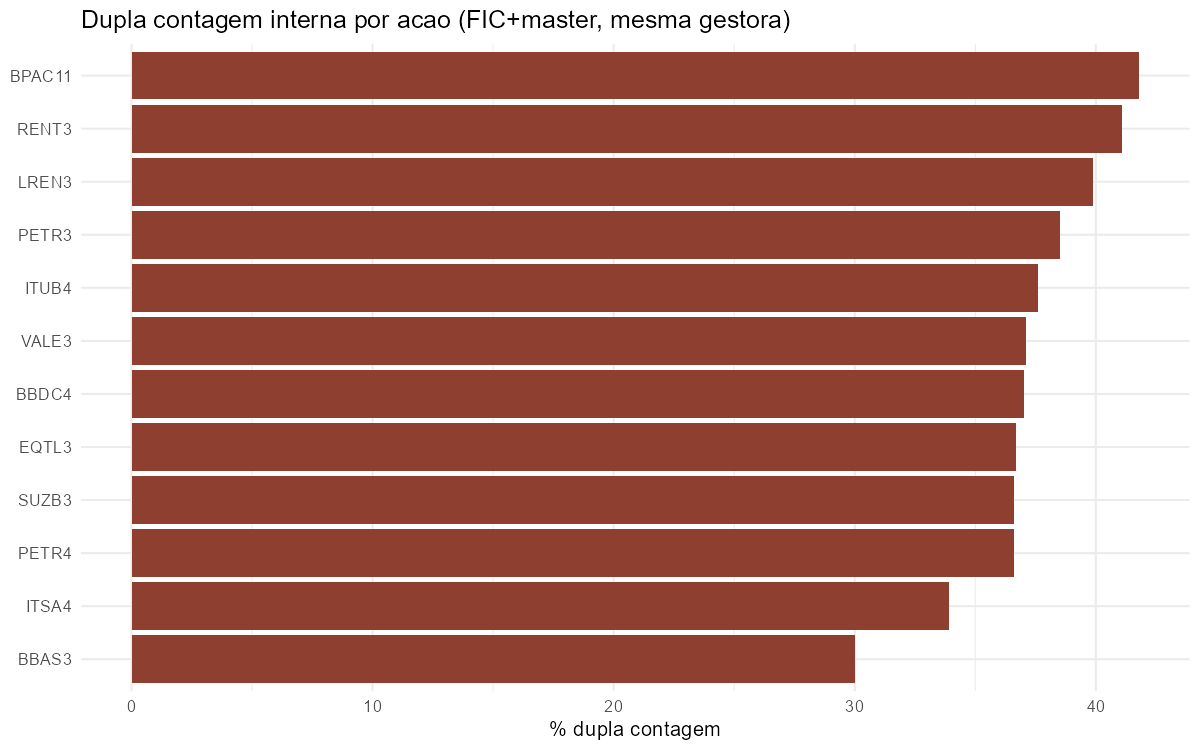
\includegraphics[width=0.8\textwidth]{dedup_pct_by_stock.png}
\caption{Percentual de dupla contagem interna (FIC$+$master da mesma gestora), por ação.}
\label{fig:dedupstock}
\end{figure}

\paragraph{Concentração de propriedade (\emph{crowding}).} A Tabela~\ref{tab:crowd} lista as ações detidas
pelo maior número de gestoras. As primeiras --- VALE3, PETR4, ITUB4, BBDC4, EQTL3, RENT3, LREN3, BRFS3,
GGBR4\ldots --- são detidas por \textbf{todas as 42 gestoras}. São exatamente os ativos sobre os quais a
\emph{demanda institucional é mais sobreposta} e, portanto, mais sujeitos à fragilidade de preços de
\citet{greenwoodthesmar2011}: um choque correlacionado de fluxos atinge todas as carteiras ao mesmo tempo.

\begin{table}[H]\centering
\caption{Ações mais ``concentradas'' (nº de gestoras detentoras; posição agregada média mensal).}
\label{tab:crowd}
\small
\begin{tabular}{lrr|lrr}
\toprule
\textbf{Ação} & \textbf{Gestoras} & \textbf{R\$ bi/mês} & \textbf{Ação} & \textbf{Gestoras} & \textbf{R\$ bi/mês} \\
\midrule
VALE3 & 42 & 10,7 & GGBR4 & 42 & 2,0 \\
PETR4 & 42 &  9,1 & CESP6 & 42 & 1,8 \\
ITUB4 & 42 &  7,1 & UGPA3 & 42 & 1,6 \\
BBDC4 & 42 &  6,9 & LAME4 & 42 & 1,6 \\
EQTL3 & 42 &  6,0 & GNDI3 & 41 & 5,9 \\
RENT3 & 42 &  4,6 & BBAS3 & 41 & 4,8 \\
LREN3 & 42 &  4,5 & SUZB3 & 41 & 4,5 \\
BRFS3 & 42 &  2,0 & & & \\
\bottomrule
\end{tabular}
\end{table}

\begin{figure}[H]\centering
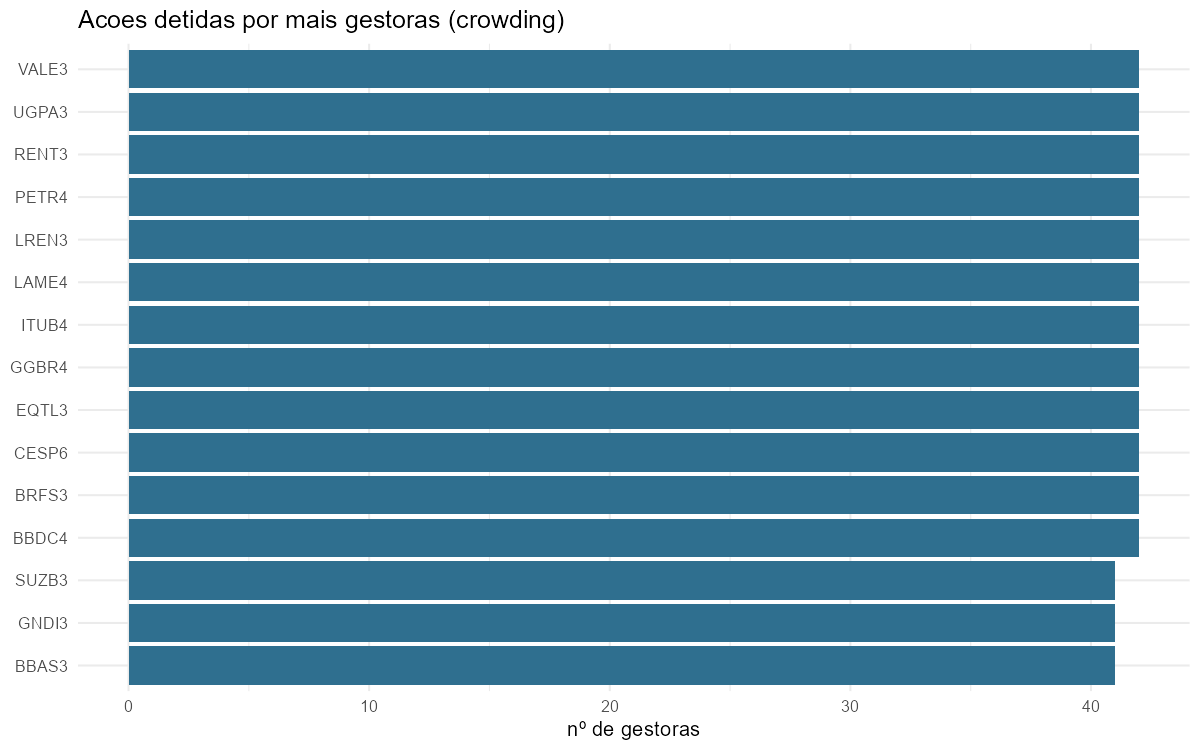
\includegraphics[width=0.8\textwidth]{stock_crowding_top15.png}
\caption{Ações detidas pelo maior número de gestoras (\emph{crowding}).}
\label{fig:crowd}
\end{figure}

\section{Discussão}\label{sec:disc}
Dois fatos se reforçam, mas em níveis diferentes de validação. No núcleo CONS+SH, a \textbf{concentração} nas
\emph{blue chips} (detidas por todas as gestoras) cria o canal de fragilidade: demanda institucional
sobreposta em ativos líquidos e comuns. Na extensão com CDA, a \textbf{duplicação $\approx 37\%$} é estável
entre ações e entre gestoras (com exceções reveladoras: Caixa, 4\%, quase não usa estruturas aninhadas; Truxt
e Atmos, $>$48\%, são intensivas em FIC). Isso sugere que somar fundos da mesma gestora sem de-duplicar pode
superestimar a exposição institucional, mas essa conclusão deve ser apresentada como resultado complementar
até a base CDA ser validada no escopo do TCC.

\section{Limitações}\label{sec:lim}
Valem as mesmas do documento principal: (i)~a exposição é net (parametrizável); (ii)~o peso é descritivo;
(iii)~na extensão CDA, parte relevante das cotas aponta para fundos externos à amostra, e o campo
\texttt{DT\_CONFID\_APLIC} exige leitura cautelosa, pois nos históricos processados o CNPJ do fundo investido
aparece preenchido mesmo quando esse campo existe. A de-duplicação reportada remove a sobreposição
\emph{intra-gestora}; não deve ser confundida com de-duplicação total do sistema.

\section{Próximos passos}\label{sec:next}
Com o painel de todas as ações e a rede fundo-sobre-fundo prontos, o passo seguinte é o \textbf{forecasting}
da variação de exposição (baselines AR/VAR, fatores latentes via PCA/análise fatorial \citep{artesbarroso2023}
e redes neurais em grafo \citep{sanchezlengeling2021}). \textbf{Nenhum modelo foi executado nesta fase.}

\bibliographystyle{plainnat}
\bibliography{refs}
\end{document}
